% !TEX root = ./document.tex

\documentclass{article}

\usepackage{mystyle}
\usepackage{myvars}

%-----------------------------

\begin{document}

  \maketitle

  %-----------------------------
  %  TEXT
  %-----------------------------

  \part{Ejercicio Kutner:\\ Mantenimiento de Copiadoras}

    \paragraph{}
    Para la realización del ejercicio de \emph{Mantenimiento de Copiadoras} mediante SAS, lo primero que se ha llevado a cabo es la importación del conjunto de datos a partir del fichero. Para facilitar dicha tarea, se ha realizado una fase previa de preprocesado para convertir el fichero a formato \texttt{csv} denotando por $Y$ la primera columna y $X$ la segunda (tal y como indica el enunciado). Una vez hecho esto, se ha utilizado el fragmento de la figura \ref{code:sas-copiers-1} para importar el conjunto de datos en \emph{SAS}. Por tanto, ya se puede comenzar a realizar el ejercicio.

    \setcounter{section}{1}
    \setcounter{subsection}{19}
    \subsection{\textbf{Copier maintenance}. The Tri-City Office Equipment Corporation sells an imported copier on a franchise basis and performs preventive maintenance and repair service on this copier. The data below have been collected from 45 recent calls on users to perform routine preventive maintenance service; for each call, $X$ is the number of copiers serviced and $Y$ is the total number of minutes spent by the service person. Assume that first-order regression model \eqref{eq:simple-linear-regression-model} is appropriate.}
    \label{sec:e1-20}

      \begin{equation}
      \label{eq:simple-linear-regression-model}
        Y_i = \beta_0 + \beta_1X_i + \epsilon_i
      \end{equation}

      \begin{itemize}
        \item $Y_i$:
        \item $\beta_0$:
        \item $\beta_1$:
        \item $X_i$:
        \item $\epsilon_i$:
      \end{itemize}


      \subsubsection{Obtain the estimated regression function.}

        \paragraph{}
        Para obtener la generación del modelo de regresión a mediante \emph{SAS} se ha utilizado el fragmento de códido \emph{SAS} de la figura \ref{code:sas-copiers-2}, que calcula los estimadores del modelo de regresión lineal simple que se ilustra en la ecuación \eqref{eq:simple-linear-regression-model}. A partir de dicha sentencia se han obtenido distintas salidas que después han sido utilizadas en otros apartados pedidos por el enunciado del problema.

        \paragraph{}
        Para la resolución de este apartado, ha sido suficiente con consultar el \say{resumen}, que se muestra en la figura \ref{img:copiers-regression-summary}, a partir de la cual se han obtenido los valores de $\beta_0$ y $\beta_1$, que se muestran en las ecuaciones \eqref{eq:beta_0} y \eqref{eq:beta_1} respectivamente.

        \paragraph{}
        Por tanto, la estimación de la función de regresión simple obtenida se muestra en la ecuación \eqref{eq:model_estimation}.

        \begin{figure}[!h]
          \centering
          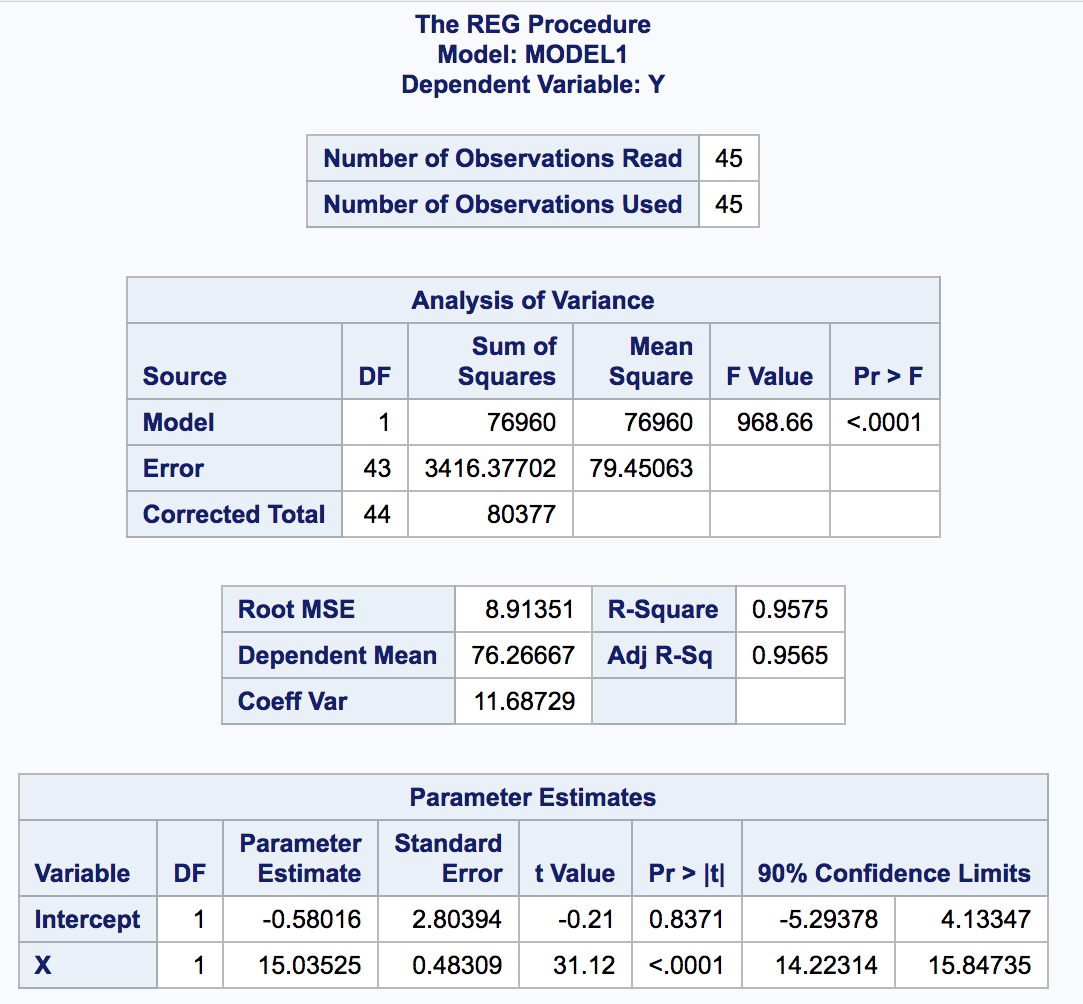
\includegraphics[width=.5\textwidth]{copiers/regression-summary}
          \caption{\emph{Salida SAS}: Mantenimiento de Copiadoras - Resumen de Regresión Lineal Simple}
          \label{img:copiers-regression-summary}
        \end{figure}

        \begin{align}
        \label{eq:beta_0}
          \widehat{\beta}_0 &= -0.58016\\
        \label{eq:beta_1}
          \widehat{\beta}_1 &= 15.03525\\
        \label{eq:model_estimation}
          \widehat{Y_i} &= \widehat{\beta}_0 +\widehat{\beta}_1X_i + \epsilon_i = -0.58016 + 15.03525 X_i + \epsilon_i
        \end{align}

      \subsubsection{Plot the estimated regression function and the data. How well does the estimated regression function fit the data?}

        \paragraph{}
        En este apartado se pide representar la recta de regresión obtenida en el apartado anterior. Afortunadamente, en este caso no ha sido necesaria la utilización de otro fragmento de código, sino que con el utilizado en el apartado anterior (figura \ref{code:sas-copiers-1}) ya se generaba dicho gráfico.

        \paragraph{}
        El gráfico en cuestión se muestra en la figura \ref{img:copiers-regression-plot}, a partir del cual se puede observar la relación lineal existente entre la variable independiente $X$ y la variable dependiente $Y$. Además, se puede apreciar como el modelo de regresió lineal simple se ajusta de manera apropiada a los datos.

        \paragraph{}
        En los siguientes apartados se analizará la dispersión de los datos así como los intervalos de confianza para la media y de predicción. Sim embargo, a simple vista y debido al contexto y unidades de medida de los datos, parece coherente el nivel de dispersión de los datos (variaciones entorno a $10$ minutos entre instalaciones).

        \begin{figure}[!h]
          \centering
          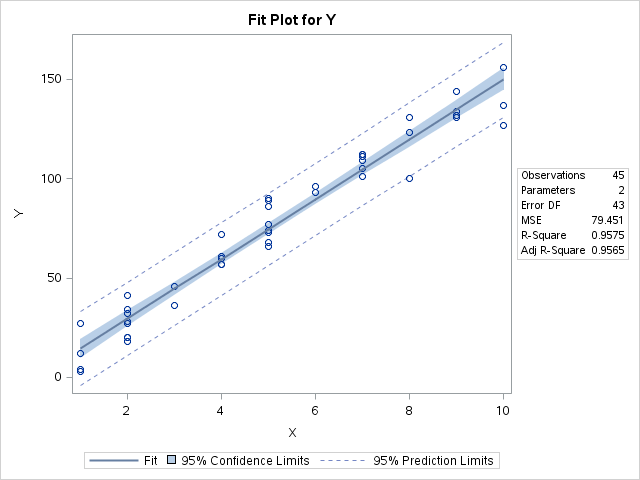
\includegraphics[width=.8\textwidth]{copiers/regression-plot}
          \caption{\emph{Salida SAS}: Mantenimiento de Copiadoras - Gráfico de Regresión Lineal Simple}
          \label{img:copiers-regression-plot}
        \end{figure}

      \subsubsection{Interpret $\widehat{\beta}_0$ in your estimated regression function. Does $\widehat{\beta}_0$ provide any relevant information here? Explain.}

        \paragraph{}
        El valor estimado de la ordenada en el origen (o \say{intercept}) se muestra en la ecuación \eqref{eq:beta_0}, el cual está muy próximo al valor $0$. La interpretación del término independiente en este caso podría ser \emph{el número de minutos que se emplean en realizar $0$ mantenimientos}, el cual tiene sentido que esté próximo a $0$ minutos.

        \paragraph{}
        Esto podría deberse a que no se contabiliza el tiempo cuando no hay mantenimiento por hacer, lo cual tiene sentido ya que el estudio trata de analizar la duración del proceso de \emph{mantenimiento de copiadoras}. Algo a destacar es que, posiblemente debido a la muestra patrón utilizada para la generación del modelo, el término independiente ha sido ajustado con valor negativo. Esto no puede tener ninguna interpretación, ya que su valor se ha ajustado de manera que el ajuste global (en términos de mínimos cuadrados) sea mínimo.

        \paragraph{}
        Tal y como se verá en el apartado \ref{sec:copiers-2.5e} del ejercicio \ref{sec:copiers-2.5}, no existen evidencias significativas para asumir que sea distinto de cero. Pero tal y como se discute en dicho apartado, no es apropiado eliminarlo ya que este haría que parte del error explicado por el modelo se convirtiese en error aleatorio, lo cual es algo negativo para el ajuste.


      \subsubsection{Obtain a point estimate of the mean service time when $X = 5$ copiers are serviced.}

        \paragraph{}
        Para la obtención de una estimación puntual para $X=5$, se ha decidido realizar el proceso de añadir una nueva observación al conjunto de datos (de manera que tan solo contenga el valor de la variable independiente $X$). Para ello, se ha utilizado el fragmento de código \emph{SAS} de la figura \ref{code:sas-copiers-3}. Nótese que esto podría haberse llevado a cabo mediante la simple sustitución del valor $X$ en la función de regresión de la ecuación \eqref{eq:model_estimation}, pero esto no nos habría ofrecido una estimación del la varianza.

        \paragraph{}
        Por tanto, la salida obtenida a través de \emph{SAS} se muestra en la figura \ref{img:copiers-regression-prediction}, la cual indica el valor predicho, así como una estimador de la desviación típica respecto de la media en ese punto. Estos valore se muestran en las ecuaciones \eqref{eq:x_5_e} y \eqref{eq:x_5_var}.

        \paragraph{}
        La interpretación que se le puede dar a dichos resultados es que para el mantenimiento de $5$ copiadoras se dedica en torno a $74.6$ minutos con una variación media de $1.15$ minutos.

        \begin{figure}[!h]
          \centering
          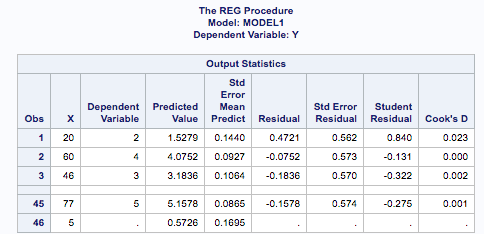
\includegraphics[width=.6\textwidth]{copiers/regression-prediction}
          \caption{\emph{Salida SAS}: Mantenimiento de Copiadoras - Prediccion de Regresión Lineal Simple para $X = 5$}
          \label{img:copiers-regression-prediction}
        \end{figure}

        \begin{align}
        \label{eq:x_5_e}
          \begin{split}
            E\left[\widehat{Y} \mid X = 5\right] &=
            E\left[\widehat{\beta}_0 +\widehat{\beta}_1X + \epsilon \mid X = 5\right]
            = -0.58016 + 15.03525 * 5 + 0 = 74.5961
          \end{split}\\
        \label{eq:x_5_var}
          \begin{split}
            Var\left[\widehat{Y} \mid X = 5\right] &=
            \sigma^2\left(1 + \frac{1}{n} + \frac{(x^* - \bar{x})^2}{S_{xx}}\right) =
            1.1531 ^ 2 =
            1.3298
          \end{split}
        \end{align}

    \setcounter{subsection}{23}
    \subsection{Refer to \textbf{Copier maintenance} Problem \ref{sec:e1-20}.}

      \subsubsection{Obtain the residuals $e_i$ and the sum of the squared residuals $\sum_i e_i^2$. What is the relation between the sum of the squared residuals here and the quantity $Q$ in \eqref{eq:least-squares-criterion}?}


        \paragraph{}
        En este apartado se pide obtener los residuos $e_i$. Para ello, se ha creido conveniente la representación de un gráfico de resiudos, el cual ha sido obtenido mediante el fragmento de código de la figura \ref{code:sas-copiers-1} utilizado en apartados anteriores.

        \paragraph{}
        Este gráfico de residuos se muestra en la figura \ref{img:copiers-regression-residuals} y a partir de él se puede apreciar una distribución más o menos uniforme de los errores (tiene cierta forma de parábola, pero esta característica es sutil). También se puede apreciar la dispersión de los datos en torno al valor $10$, tal y como se indicó en partaados anteriores.

        \begin{figure}[!h]
          \centering
          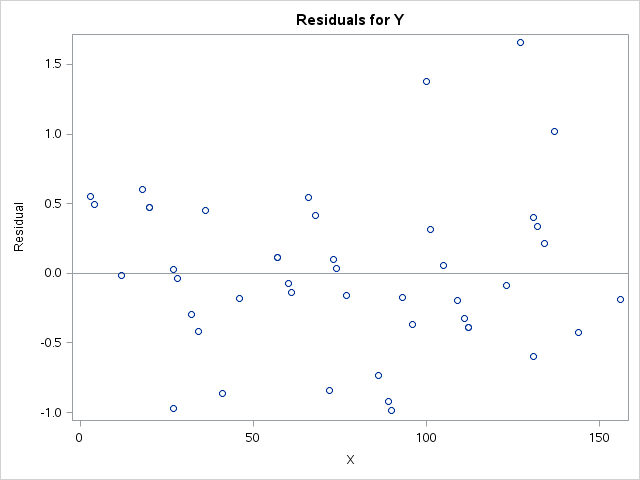
\includegraphics[width=.8\textwidth]{copiers/regression-residuals}
          \caption{\emph{Salida SAS}: Mantenimiento de Copiadoras - Gráfico de Residuos de Regresión Lineal Simple}
          \label{img:copiers-regression-residuals}
        \end{figure}

        \begin{equation}
        \label{eq:least-squares-criterion}
          Q = \sum\limits_{i=1}^n(Y_i - \beta_0 - \beta_1X_i)^2 = 3416.37702
        \end{equation}

        \paragraph{}
        En el título del apartado, también se pide el valor de la suma de errores al cuadrado $\sum_i e_i^2$, así como su relación con el valor $Q$, que se muestra en la ecuación \eqref{eq:least-squares-criterion}. El valor $Q$ es aquel que se trata de minimizar bajo el criterio de mínimos cuadrados en el modelo de regresión simple. Este ha sido extraido del resumen generado por \emph{SAS}, que se muestra en la figura \ref{img:copiers-regression-summary} utilizada en otros apartados.

        \paragraph{}
        Por tanto, es la medida del error en términos de mínimos cuadrados de la recta de regresión obtenida con respecto del conjunto de datos. sto puede escribirse como $Q = \sum_{i=1}^n(Y_i - \widehat{Y}_i)^2$, y dado que los errores $e_i$ se definen como $Y_i - \widehat{Y}_i$ la equivalencia es directa, es decir, $Q = \sum_i e_i^2$.

      \subsubsection{Obtain point estimates of $\sigma^2$ and $\sigma$. In what units is $\sigma$ expressed?}

        \paragraph{}
        En este apartado se han pedido obtener estimaciones acerca de la dispersión de los errores, es decir, del valor $\sigma$. Al igual que en anteriores apartados, este valor se ha obtenido a partir del código \emph{SAS} de la figura \ref{code:sas-copiers-1}, que ha generado los resultados obtenidos en la figura \ref{img:copiers-regression-summary}.

        \paragraph{}
        La varianza y la desviación típica de los errores se muestran en las ecuaciones \eqref{eq:sigma-2} y \eqref{eq:sigma} respectivamente. En el título del apartado se indica además que se explique cuáles son las unidades de medida de la desviación típica de los errores $\sigma$. Es sencillo entender que las unidades de esta medida serán en \emph{minutos}, ya que esta mide la dispersión de los datos en torno a la predicción obtenida por la recta de regresión, la cual se refiere a la variable dependiente $Y$, que representa el número de minutos en realizar el mantenimiento.

        \begin{align}
        \label{eq:sigma-2}
          \begin{split}
            \widehat{\sigma}^2 &= MSE = \frac{SSE}{n-2} = \frac{\sum_{i=1}^n(Y_i - \widehat{Y}_i)^2}{n-2} = \frac{3416.37702}{45-2} = 79.45063
          \end{split} \\
        \label{eq:sigma}
          \begin{split}
            \widehat{\sigma} &= \sqrt{\widehat{\sigma}^2} = \sqrt{79.45063} = 8.91351
          \end{split}
        \end{align}

    \setcounter{section}{2}
    \setcounter{subsection}{4}
    \subsection{Refer to \textbf{Copier maintenance} Problem \ref{sec:e1-20}.}
    \label{sec:copiers-2.5}

      \subsubsection{Estimate the change in the mean service time when the number of copiers serviced increases by one. Use a $90\%$ confidence interval. Interpret your confidence interval.}
      \label{sec:copiers-2.5a}

        \paragraph{}
        [TODO]

        \begin{align}
          t_{n-2;1-\frac{\alpha}{2}} &= t_{43;0.95} = 1.681071\\
          Var\left[\widehat{\beta}_1\right] &= 0.23337
        \end{align}

        \begin{equation}
          \text{I.Conf.}
          = \left[\widehat{\beta}_1 \pm t_{n-2;1-\frac{\alpha}{2}}\sqrt{Var\left[\widehat{\beta}_1\right]}\right]
          = \left[15.03525 \pm 0.8121\right]
          = \left[14.2232, 15.8474\right]
        \end{equation}

      \subsubsection{Conduct a \emph{t-test} to determine whether or not there is a linear association between $X$ and $Y$ here; control the $\alpha$ risk at $0.10$. State the alternatives, decision rule, and conclusion. What is the \emph{P-value} of your test?}
      \label{sec:copiers-2.5b}

        \paragraph{}
        [TODO ]

        \begin{equation}
          \begin{split}
            H_0&: \beta_1 = 0 \\
            H_1&: \beta_1 \neq 0
          \end{split}
        \end{equation}

        \begin{equation}
            \text{p-value}
            = 2Pr\left[\abs{\frac{\widehat{\beta}_1 - 0}{\sqrt{Var\left[\widehat{\beta}_1\right]}}} > t_{n-2}\right]
            = 2Pr\left[\frac{15.03525}{0.48309} > t_{43}\right]
            = 2Pr\left[31.12 > t_{43}\right]
            < 0.0001
        \end{equation}


      \subsubsection{Are your results in parts (\ref{sec:copiers-2.5a}) and (\ref{sec:copiers-2.5b}) consistent? Explain.}

        \paragraph{}
        [TODO ]

      \subsubsection{The manufacturer has suggested that the mean required time should not increase by more
than $14$ minutes for each additional copier that is serviced on a service call. Conduct a test to decide whether this standard is being satisfied by Tri-City. Control the risk of a Type I error at $0.05$. State the alternatives, decision rule, and conclusion. What is the \emph{P-value} of the test?}

        \paragraph{}
        [TODO ]

        \begin{equation}
          \begin{split}
            H_0&: \beta_1 \leq 14 \\
            H_1&: \beta_1 > 14
          \end{split}
        \end{equation}


        \begin{equation}
            \text{p-value}
            = Pr\left[\frac{\widehat{\beta}_1 - 14}{\sqrt{Var\left[\widehat{\beta}_1\right]}} > t_{n-2}\right]
            = Pr\left[\frac{1.03525}{0.48309} > t_{43}\right]
            = Pr\left[2.14297 > t_{43}\right]
            = 0.01890824
        \end{equation}


      \subsubsection{Does $\widehat{\beta}_0$ give any relevant information here about the start-up time on calls-i.e., about the time required before service work is begun on the copiers at a customer location?}
      \label{sec:copiers-2.5e}
        \paragraph{}
        [TODO ]

        \begin{equation}
          \begin{split}
            H_0&: \beta_0 = 0 \\
            H_1&: \beta_0 \neq 0
          \end{split}
        \end{equation}

        \begin{equation}
            \text{p-value}
            = 2Pr\left[\abs{\frac{\widehat{\beta}_0 - 0}{\sqrt{Var\left[\widehat{\beta}_0\right]}}} > t_{n-2}\right]
            = 2Pr\left[\abs{\frac{-0.58016}{2.80394}} > t_{43}\right]
            = 2Pr\left[\abs{-0.21} > t_{43} \right]
            = 0.8371
        \end{equation}

    \setcounter{subsection}{13}
    \subsection{Refer to \textbf{Copier maintenance} Problem \ref{sec:e1-20}.}

      \subsubsection{Obtain a $90\%$ confidence interval for the mean service time on calls in which six copiers are serviced. Interpret your confidence interval.}
      \label{sec:copiers-2.14a}


      \begin{figure}[!h]
        \centering
        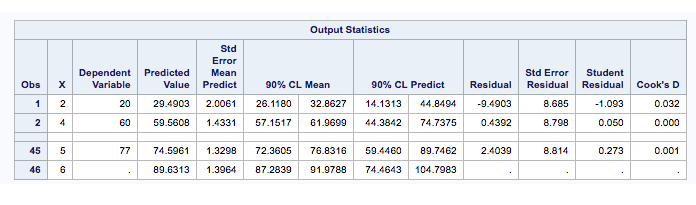
\includegraphics[width=.85\textwidth]{copiers/regression-prediction2}
        \caption{\emph{Salida SAS}: Mantenimiento de Copiadoras - Prediccion de Regresión Lineal Simple para $X = 6$}
        \label{img:copiers-regression-prediction2}
      \end{figure}

        \paragraph{}
        [TODO ]

        \begin{align}
          \widehat{Y}_h &= \widehat{\beta}_0 +\widehat{\beta}_16+ \epsilon_h = 89.6313\\
          t_{n-2;1-\frac{\alpha}{2}} &= t_{43;0.95} = 1.681071\\
          Var\left[\widehat{Y}_h \right]  &= 1.9499
        \end{align}

        \begin{equation}
          \text{I.Conf.}
          = \left[\widehat{Y}_h \pm t_{n-2;1-\frac{\alpha}{2}}\sqrt{Var\left[\widehat{Y}_h \right]}\right]
          = \left[89.6313 \pm 2.3475\right]
          = \left[87.2839, 91.9788\right]
        \end{equation}

      \subsubsection{Obtain a $90\%$ prediction interval for the service time on the next call in which six copiers are serviced. Is your prediction interval wider than the corresponding confidence interval in part (\ref{sec:copiers-2.14a})? Should it be?}

        \paragraph{}
        [TODO ]

        \begin{align}
          \widehat{Y}_{pred} &= \widehat{\beta}_0 +\widehat{\beta}_16 + \epsilon_i = 89.6313\\
          t_{n-2;1-\frac{\alpha}{2}} &= t_{43;0.95} = 1.681071\\
          Var\left[\widehat{Y}_{pred}\right] &= \widehat{\sigma}^2 + Var\left[\widehat{Y}_h \right]  =79.45063 + 1.9499 = 81.40053
        \end{align}

        \begin{equation}
          \begin{split}
            \text{I.Pred.}
            = \left[\widehat{Y}_{pred} \pm z_{1-\frac{\alpha}{2}}\sqrt{Var\left[\widehat{Y}_{pred}\right]}\right]
            = \left[89.6313 \pm 15.167\right]
            = \left[74.4643, 104.7983\right]
          \end{split}
        \end{equation}


    \setcounter{subsection}{23}
    \subsection{Refer to \textbf{Copier maintenance} Problem \ref{sec:e1-20}.}

      \setcounter{subsubsection}{1}
      \subsubsection{Conduct an \emph{F-test} to determine whether or not there is a linear association between time spent and number of copiers serviced; use $\alpha = 0.1$. State the alternatives, decision rule, and conclusion.}

        \paragraph{}
        [TODO ]

        \begin{equation}
          \begin{split}
            H_0&: \beta_1 = 0 \\
            H_1&: \beta_1 \neq 0
          \end{split}
        \end{equation}

        \begin{equation}
          \text{p-value} = Pr\left[\frac{MSM}{MSE} > F_{1;n-2}\right] =
          Pr\left[\frac{76960}{79.45063} > F_{1;43}\right] =
          Pr\left[968.66 > F_{1;43}\right] <
          0.0001
        \end{equation}

      \subsubsection{By how much, relatively, is the total variation in number of minutes spent on a call-reduced when the number of copiers serviced is introduced into the analysis? Is this a relatively small or large reduction? What is the name of this measure?}

        \paragraph{}
        [TODO coeficiente de determinación]

        \begin{equation}
          R^2 = \frac{SSM}{SST} = \frac{76960}{76960 + 3416.37702} = 0.9574
        \end{equation}

      \subsubsection{Calculate $r$ and attach the appropriate sign.}

        \paragraph{}
        [TODO ]

        \begin{equation}
          r = + \sqrt{R^2} = 0.9785
        \end{equation}

  \part{Ejercicios Montgomery:}

    \paragraph{}
    [TODO ]


  \part{Código Fuente}

    \begin{figure}[!h]
      \centering
      \begin{minted}[frame=single,framesep=5pt]{sas}
filename reffile '/folders/myshortcuts/sas/regression-group-task/data/CH01PR20.csv';

proc import datafile=reffile dbms=csv out=copiers;
  getnames=yes;
run;

proc print data=copiers;
run;
      \end{minted}
      \caption{\emph{Código SAS:} Mantenimiento de Copiadoras - Importación del conjunto de datos.}
      \label{code:sas-copiers-1}
    \end{figure}


    \begin{figure}[!h]
      \centering
      \begin{minted}[frame=single,framesep=5pt]{sas}
proc reg data=copiers;
  model y=x;
  id x;
run;
      \end{minted}
      \caption{\emph{Código SAS:} Mantenimiento de Copiadoras - Modelo de regresión simple.}
      \label{code:sas-copiers-2}
    \end{figure}

    \begin{figure}[!h]
      \centering
      \begin{minted}[frame=single,framesep=5pt]{sas}
data copiers_new_observation;
  x = 5;
run;

proc append base=copiers data=copiers_new_observation;
run;

proc reg data=copiers;
  model y = x /r clm;
  id x;
run;
      \end{minted}
      \caption{\emph{Código SAS:} Mantenimiento de Copiadoras - Predicción para $X = 5$.}
      \label{code:sas-copiers-3}
    \end{figure}

    \begin{figure}[!h]
      \centering
      \begin{minted}[frame=single,framesep=5pt]{sas}
data copiers_new_observation;
  x = 6;
run;

proc append base=copiers data=copiers_new_observation;
run;

proc reg data=copiers;
  model y = x /r cli clm alpha=0.1;
  id x;
run;
      \end{minted}
      \caption{\emph{Código SAS:} Mantenimiento de Copiadoras - Predicción para $X = 6$.}
      \label{code:sas-copiers-4}
    \end{figure}

  %-----------------------------
  %  Bibliographic references
  %-----------------------------

  \nocite{rano2017}
  \nocite{sas}
  \nocite{neter1996applied}
  \nocite{montgomery2012introduction}

  \bibliographystyle{acm}
  \bibliography{bib}

\end{document}
